\section{Simulation System Engineering}\label{methodology-software}

\subsection{Requirements}

Based on the results and findings of the experiments presented in section \ref{methodology-basic}, we have come with a set of requirements for the next iteration of our simulation system.

It was decided to drop the older IveTrainer software in favour of developing a new system from ground up. IveTrainer was aimed to be a well scalable and extendable simulation system, but during the development many of the features were constructed in a poorly extendable way.

The updated software needs to adopt industry standard software design techniques. The software developed during this project also adheres to the `good' programming practices. Improved modularity and high coherence leads to unconstrained testing and functionality extension.

The new version of the system is required to be much more scalable and portable. The system is also required to include support for more sophisticated physical models.

\subsection{BirthEngine with .NET/Mono}

The .NET framework for the first iteration of reimplementing the simulation software. The new version of the software was named BirthEngine.

\subsubsection{Crossplatform runtime}
  The Mono Framework \citep{mono_framework} is a cross-platform implementation of Microsoft's .Net framework that allows building and deploying .Net applications on platforms other than Microsoft Windows. By utilizing the framework the BirthEngine simulation system is capable of being run on multiple platforms.

\subsubsection{Rendering capabilities}

  Simulation systems often lack the appealing rendering capability of the more graphics oriented applications, such as games. However, we believe that having a realistic graphical representation of the simulation environment carries a great role in immersiveness of the scene, which in turn affects how effective the training is. Therefore, a considerable attention is given the graphical engine of the simulations sytem.

  OpenTK \citep{opentk} is an open-source toolkit that wraps around a number of low level API's. It provides access to the OpenGL, OpenAL and OpenCL API's of the target platform. OpenTK was used in developing the graphical component of the simulation system.

  The IveTrainer rendering engine was based on the less efficient OpenGL 2.0 API. The OpenGL 3.0 is used. The choise of using the third version of the API instead of the latest OpenGL 4.0 is justified by the requirement of backwards capability. The simulation system is inteded to work even on a less modern hardware, which will not necessarily support the latest OpenGL API.

  The chosen API is sufficiently modern to allow more realistic and efficient rendering capabilities. The list of .

  \begin{itemize}
    \item Shaders based rendering for a highly customizable rendering capabilities
    \item Deferred shading for efficient multi-light scenes
    \item Volumetric rendering of voxel data using ray-tracing in shaders
    \item Vertex Buffer Object based mesh rendering to minimize memory transfer times for increased rendering speeds
  \end{itemize}

  The rendering engine of BirthEngine is build around the low level API to allow easier and faster creation of graphical representation of simulations. Object-oriented abstractions are built on top of the \'C like\' API.

\subsubsection{Entity Component System}

Entity component system (ECS) is a popular framework primarily used in high-performance oriented graphical applications development, particulary in game development. The framework is an example of a broader approach to software engineering known as \textit{Composition Over Inheritance}. The approach is a well known design pattern and can be found in the book \citep{Freeman:2004:HFD:1076324}.

ECS is chosen as the core approach to describing the simulation elements and their behaviours. The main idea is that each simulation object is represented by an \textit{entity}. Note that all scene elements are entities directly and not through inheritance.

The class diagram in Figure \ref{software-ecs} provides an example of how ECS is used to represent a part of a simulation scene. The object

\begin{figure}
\begin{center}
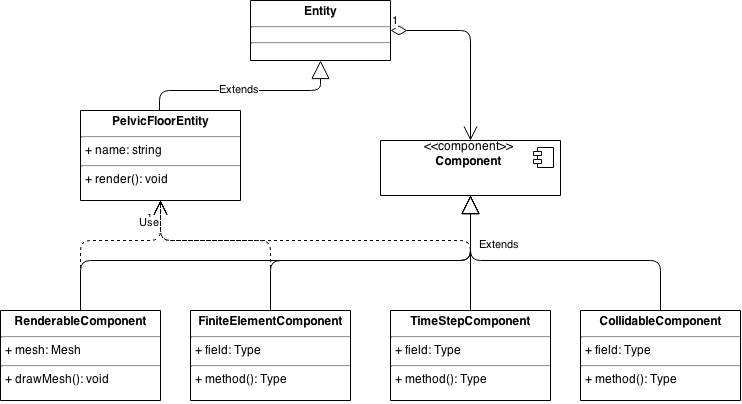
\includegraphics[width=100mm]{sections/methodology/images/software/software-ecs.png}
\caption[Entity component system use in BirthEngine.]{\label{software-ecs} Entity component system use in BirthEngine.}
\end{center}
\end{figure}
